\documentclass[12pt]{article}
\usepackage{graphicx}
\usepackage{pstricks}
\usepackage[letterpaper,pdftex,right=1in,left=1in,top=1in,bottom=1in]{geometry}
\usepackage{amsmath}
\usepackage{amsthm}
\usepackage{amssymb}
\usepackage{setspace}
\usepackage{multirow}
\usepackage{hyperref}
\usepackage{lscape}
\usepackage{booktabs}
\usepackage{enumitem}
\renewcommand{\bibitem}{\vskip
2pt\par\hangindent\parindent\hskip-\parindent}
\renewcommand{\baselinestretch}{2.0}

\title{Geostatistical Analysis in Space and Time}
\author{Logan Stundal, Benjamin Bagozzi, and John Freeman}
% ---------------------------------------------------------------------------- %


\begin{document}
\maketitle
\doublespace


% ---------------------------------------------------------------------------- %
% INTRODUCTION
% ---------------------------------------------------------------------------- %
Spatial temporal processes are at the heart of many important political questions. How do ideologies of mass publics evolve within and across state boundaries? How does electronic media affect the attitudes and behavior of citizens over time within counties in different states, attitudes and behaviors which through political communication diffuse to and from neighboring counties? How do candidates decide where and when to to raise funds (``search for gold") in their constituencies? How do their efforts spawn new contributions over time from locations outside their constituencies? Why and how do civil wars break out in and then spread across governmental jurisdictions dying out in some places but escalating in others?

Political methodology lags behind other disciplines like criminology, meteorology, environmental
science, and epidemiology in its analysis of spatial temporal processes. We have made
real advances in spatial measurement (Monogan and Gill 2015; Cho 2003), causal inference based
on geographical designs (Keele and Titiunik 2015) and the study of conflict
dynamics (Brandt, et al 2008, 2014). But, many of our spatial analysis ignore or
downplay temporal factors; they assess treatment effects at a single point in time. Or, we
study spatial processes but in separate or highly aggregated slices of time (Cho and Gimpel 2007).
Leading textbooks on time series in political science and economics
(Box Steffensmeier et al. 2014, Enders 2010) say nothing about spatial-temporal
processes. Difference-in-difference causal analysis use two time points to
make grand assumptions about time trends in
complex political process without any provision for medium and long term dynamics, \
let alone diffusion across (omitted) units of analysis (Keele and Minozzi 2013).
Many conflict studies are macro-level investigations in which spatial factors
amount to country dyadic exchanges or exchanges between  belligerents (Brandt et al. 2008). Subnational
conflict studies make a ``localization" assumption--that conflict occurs over time within
but not across units of analysis (Silverman 2021).

If they allow for spatial temporal factors in their analysis, political scientists most
often place two way fixed effects in their models and, concomitantly, used cluster errors
to account for any remaining unit heteroscedasticity. Occasionally, a
simple (static) spatial model is used to assess the robustness of the
investigator's results. As we explain below, conceptually, two way fixed effects models
do not allow for diffusion of the effects of the variables of interest across
units and they treat the effect of ``time" as identical on all units in each
time slice; two way fixed effects set-ups ignore the possibility of individual
space-time unit differences in the effects of causal mechanisms.

Some of us have applied and made advances in neighborhood type spatial temporal
modeling. These modelers carve up space into discrete units and include in regression
models right hand side variables with both spatial lags with \emph{prespecified}
connectivity matrices of the dependent variable and also
temporal lags of the values of the own unit's past values
of the dependent variable. The development of such models for binary dependent
variables along with techniques to assess spatial and temporal marginal effects
is illustrative (Ward and Gleditsch 2002, Franzese et al. 2015). An innovative application
of spatial vector autoregression in the study of subnational conflict also has
been applied in international relations (Linke et al. 2012).

With one or two exceptions, what has not been applied and developed in political science,
is the  geostatistical approach to spatial temporal analysis. This approach treats
the data generating process as continuous in space; it employs a set of techniques
for "point process" modeling. Rather prespecifying a connectivity matrix, the
geostatistical approach \emph{estimates} the extent of spatial interdependence
between units and allows for unit variant temporal evolution of causal mechanisms
like diffusion. Out of the geostatistical approach emerges methods for tracking
\textit {the distinct effects of causal mechanisms for every individual unit at each point
in time.} Its is this methodology that has proven so useful recently in other
disciplines.\footnote{Geostatistical modeling is mentioned as a possible
approach in one paragraph at the end of the second edition of Ward and Gleditsch
(2019). And it has been applied in the form of kriging by
by Monogan and Gill 2015, Gill 2020, Cho and Gimpel 2007. But these studies are
static in character. The spatial-temporal versions of kriging, what is
called, co-kriging, to our knowledge,
have not been applied by American political methodologists. But see
Pavia et al. 2008.}

This research note explains a popular geostatistical approach and compares it to
the more familiar two way fixed effects and neighborhood methods of modeling
spatial temporal processes. We begin by reviewing the ways two familiar
methods conceive of spatial temporal processes. The key idea of
separability is introduced in this context. Geostatistical modeling based
on a stochastic partial differential equation then is introduced.
A formal definition of separability and the additional concepts of
space-time stationarity and isotropy are discussed briefly here.
 We then the compare the three approaches. We
use the modeling of insurgent attacks in Iraq -- in particular, Silverman's
recent (2021) two way fixed effects based investigation -- as our benchmark.
As an added payoff of our analysis, we compare the modeling results for
ground truth (army reported SIGACTS), machine coded (ICEWS) and human
coded (GED) databases; the rationale for our comparison of the databases
is explained elsewhere (Bagozzi et al. 2018; Stundal et al. forthcoming).

We find support for moving beyond static approaches to addressing space and time in our model. The results we present here demonstrate the benefit of incorporating dynamics into our analyses either with pre-specified structural models of spatiotemporal processes or through novel geostatistical frameworks which treat spatiotemporal mechanisms as a latent process.
% ---------------------------------------------------------------------------- %



% ---------------------------------------------------------------------------- %
\section{Geostatistical Modeling Spatial Temporal Processes}
% ---------------------------------------------------------------------------- %
Spatial temporal modeling is motivated by theoretical expectations, predictions, and empirical observations which suggest the existence of certain causal mechanisms: as regards space, the possibility
of strategic interaction, diffusion, spillover, relocation, and advection and as regards time, persistence,
cumulation, and memory. Spatial temporal models aim to capture the \emph{combination} of
such mechanisms. The notion that civil conflict in a particular location in one part of country not only
spills over to another part of the same or neighboring countries contemporaneously and
historically at the same time the conflict persists (is remembered) within the unit in
which it originated is illustrative. Schutte and Weidmann (2011) are among those who explain why
spatial-temporal interdependence should be expected in civil conflicts. They detect evidence
of ``escalation diffusion" in the Bosnian, Burundi, and Rwandan cases.

Two way fixed effects set ups are among the most common approaches political scientists use
to study spatial temporal political processes. Assume we observe $i = 1 \dots N$ units at $t= 1 \dots T$ points
in time. And we are interested in the effect of a set of covariates, $X_{kit}$ on variable $Y_{it}$.
This most simple model is of the form
\begin{equation}
Y_{it} = \alpha_i + \gamma_t + \beta X_{it} + \epsilon_t
\end{equation}

where $Y_{it}$ is an Nx1 dependent variable vector, $X_{kit}$ is a Nxk matrix of
covariates, $\alpha_i$ is the fixed (time invariant) affect of factors at each location i,
$\gamma_t$ is the fixed (unit invariant) affect of unknown factors at each respective
time point, $\beta$ is a coefficient vector to be estimated and $\epsilon_{it}$ is a Nx1 error
vector which may be heteroscedastic. The fixed effects are separated and added together.
There is no provision for interdependence between the values of $Y_{it}$ of any units,
there is no persistence or other kinds of temporal mechanisms governing the evolution
of $Y_{it}$, and there is no variation in the impact of historical factors across units at each
point in time.\footnote{Other simple models are used in political science such as the unit fixed
effects model with a lagged outcome variable, $Y_{it}= \alpha_i + \beta X_{kit} + \rho Y_{i, t-1} +
\epsilon_{it}$. And more complete representations of the effect of history are often employed
such as time polynomials. But, again, these alternative set ups ignore the possibility of
spatial interdependence and treat the effect of history as unit invariant. On the latter
point see the discussion Franzese et al. 2015 esp. pps. 152 and 165.}

A second, familiar model is the so-called Spatial Temporal Autoregressive (STAR) Neighborhood
model. These are usually expressed as

\begin{equation}
Y_{it} = \rho W Y_{t} + \phi M Y_{i,t-1} + \beta X_{kit} + \epsilon_{it}
\label{equation:star}
\end{equation}

As Franzese et al. (2007: 159) explain, W is the
Kronecker product of a TxT identity matrix and an NxN prespecified spatial weights matrix
$(I_t \bigotimes W_N)$, M is an NTxNT matrix of zeros except for ones on the minor
diagonal at coordinates (N+1,1), (N+2,2) ...(NT,NT-N), $\rho$ is the time invariant spatial autoregressive coefficient, and $\phi$ is the unit invariant
temporal autoregressive coefficient. Anselin (2006: Section 26.2.1)) argues that this set-up captures
diffusion, persistence and the other causal mechanisms enumerated above. The first term on the right represents
spatial interdependence while the second term captures unit persistence and related
temporal factors. Again, these factors are assumed to be separable and additive.\footnote
{There is a related model that according to Anselin and others is best suited to
analyzing spatial connections in the errors. Stundal et al. (2021) argue that conceptually, the
spatial error model (SEM)for answering our questions about
the validity of human and machine coded event data. SEMs capture model errors for
neighboring units that cluster together---``smaller(larger) errors for observation $i \ldots$
go together with smaller [larger] errors for [neighbor] $j$" (Ward and Gleditsch 2019: 76).
Errors also may be correlated because of the mismatch between the spatial scale of a process
and the discrete spatial units of observations (Anselin 2006: 907). These error patterns
correspond respectively to what researchers call the remoteness problem. For example,
remoteness means that a model's underestimates of violence in a unit distant from a
capital city correlate with underestimates of violence in a neighboring unit which is
also distant from the same city. An example, is the spatial probit error model, SPEM.
A technique based on the conditional log likelihood and variance-covariance matrix of
the model can be used to estimate it (Martinelli and Geniaux 2017). The model provides
estimates of a $\lambda$ parameter which, with a row-standardized connectivity matrix,
indicates the average dependence in the errors of a prespecified set of neighbors on
the estimation error in a unit of interest.} Solving the reduced form of Equation \ref{equation:star} yields $Y_{it} = (I - \rho W - \phi M)^{-1} * \beta X_{kit} + \epsilon_{it}$ which implies dynamic feedback effects across space and over time to unit-changes in the exogenous factors.

Neighborhood models may suffer from ``inappropriate discretization" (Lindgren and Rue 2015: 3).
The prespecified connectivity matrices used in neighborhood models treats spatial dependence
as a step function---the same for some subset of units and nonexistent for another subset of
units. The same is true of methods used to detect spatial-temporal interdependence such as
that developed by Schutte and Weidmann (2011) who use a ``Moore neighborhood" to assess
escalation diffusion and relocation. In reality the spatial dependence may vary \textit{continuously}
in space.  The alternative---geostatistical spatial error models---produce \textit{estimates}
of both the range of spatial error dependence and of the site specific impact of unobserved
factors.

Geostatistical models analyze point referenced data. These models are based on the idea of a
continuous spatial domain. For example, even though terrorist events are observed at specific
locations and therefore ``inherently discrete" these events are interpreted as realizations of
a continuously indexed space-time process of violence perpetrated against civilians and
government officials (Python et al. 2017, 2018). Formally, the data are defined by a
process indexed in time and space:
$Y(s,t) \equiv [y(s,t), (s,t) \in D \subset R^2 x R)$. The spatial-temporal covariance function
for the process is written as $Cov(y(s_i,t)y(s_j,u)) = C(y_{it},y_{ju})$. Under an assumption
of stationarity in space and time (see below) the covariance function can be expressed in terms of a combination
of spatial distance, $\Delta_{ij} = ||s_i - s_j||$, and temporal lag $\Lambda_{tu} = |t-u|$.
Thus $Cov(y_{i},y_{ju}) =
 C(\Delta_{ij}, \Lambda_{tu}).$ \footnote{As regards the spatial location of the data,
 $s$, can vary continuously in a fixed domain;
 $s$ is a two-dimensional vector with latitudes and longitudes (three-dimensional if
 altitudes are considered) This definition of the process is taken from Blangiardo
 and Cameletti 2015: 235-236.}

As in neighborhood modeling, several concepts are especially important in geostatistical
analysis. First, as in the fixed effects models and STAR setups, spatial and temporal
factors often are assumed to be \emph{separable}. This means that covariance function can be written as a
sum or product of its spatial and temporal parts,
for instance, $Cov(y_{it},y_{ju}) = C_1(\Delta_{ij})C_2(\Lambda_{tu})$. Gneiting (2002) proposes
a test for separability for modeling spatial-temporal data.\footnote{Harvill (2010: 375) explains
that ``covariance functions imply that small changes in the locations of
observations can lead to large changes in the correlations between certain linear combinations
of observations."}
\textit{Stationarity} is a second key concept. Stationarity in space implies that mean function of
the process is constant in space and that the spatial covariance function depends only on the
distance vector $s_i - s_j \in R $. A closely related concept is \emph{isotropy}; this is the
idea that the covariance function depends only on
Euclidean distance, $||s_i - s_j|| \in R$ (rotational invariance). For instance,
 Bandyopadhyay and Rao (2017) provide a test for
stationarity for irregularly spaced data.  In time series analysis stationarity means, roughly, that the mean and
all its autocovariances are unaffected by a change in its time origin. The Dickey Fuller
test is an example of a test for nonstationarity.  Because time is ordered and space is not,
isotropy has no meaning in the spatial-temporal context (Harvill 2010: 375).\footnote{Technically
this definition of spatial stationarity is a definition of second order stationarity.
``Formally, the spatial process is
a Gaussian field if for any $n \geq 1$ and for each set of locations $(s_1, \ldots, s_n)$ the
vector $(y(s_1), \dots, y(s_n)$ follows a multivariate Normal distribution with mean
$\mu = (\mu(s_1) \ldots, \mu(s_n)$  and spatially structured covariance matrix $\Sigma$.
[Then in terms of the notation in the text above] the spatial process is second order
stationary if the mean function is constant in space, i.e., $\mu(s_i) = \mu$ for each i and
the spatial covariance function depends only on the distance vector $(s_i- s_j) \in R^2$"
(Blangiardo and Cameletti 2015: 193. In atmospheric
studies second order stationarity might be violated due to topological factors. Jun and
Cook (2020) propose to model
terrorism and related phenomenon as nonstationary processes. As regards the temporal
part of the process, let $y_t$ be a time series. Then this series is \textit{covariance
stationary} if for all t and t-s,
\begin{equation}
E(y_t) = E(y_{t-s}) = \mu
\end{equation}

\begin{equation}
E(y_t - \mu)^2 = E[(y_{t-s} - \mu)^2] = \sigma_{y}^2 \\, \hspace{1cm} var(y_t) = var (y_{t-s}) = \sigma_{y}^2
\end{equation}
\begin{equation}
E[(y_t - \mu)(y_{t-s} - \mu)] = E[(y_{t-j} - \mu)(y_{t-j-s} - \mu)] = \gamma_s \\
\end{equation}
where $\mu, \sigma_{y}^2$, and  $\gamma_s$ are all constants (Enders 2010: 64). Financial
time series and, according to some scholars, approval of the President, are
nonstationary.}

A popular geostatistical approach is Continuous
Domain Bayesian Modeling with Integrated, Nested Laplacian Approximation
(INLA).\footnote{The following description draws from Blangiardo and Cameletti (2015: Chapter 6)
and especially the passage on pps. 234-5 of Python et al.\ (2017). Extensions that allow for
modeling nonstationary processes are
reviewed Ingebritsen  et al. (2015). } Briefly, this approach ``does not build models solely
for \emph{discretely observed data} but for approximations of \emph{entire processes} defined
over continuous domains" (Lindgren and Rue 2015:3, emphasis in the original). It assumes that
 the data generating process is a Gaussian field, $\xi(s)$, where $s$ denotes a finite set of
 locations, $(s_1 \ldots s_m)$. As such it suffers from a ``big n problem;" analyzing the
 Gaussian field is costly computationally (Lindgren et al. 2011). Therefore, a particular
 linear, stochastic partial differential equation is assumed to apply to the Gaussian field:

\begin{equation}
  (\kappa^2 - \Delta)^{\frac{\alpha}{2}}(\tau \xi (s)) = W(s), \hspace*{1cm} s \in D
\end{equation}
\noindent where $\Delta$ is a Laplacian,  $\alpha$ is a smoothness parameter such that
$\alpha = \lambda + 1$ (for two dimensional processes), $\kappa > 0$ is a scale parameter,
$\tau$ is a precision parameter, the domain is denoted by $D$, and $W(s)$ is Gaussian spatial
 white noise. The stationary solution to this equation is a Gaussian field with the
 Mat\'{e}rn covariance function:

\begin{equation}
  Cov(\xi(s_i),\xi(s_j)) = \sigma^2_{\xi_i}\frac{1}{\Gamma(\lambda)2^{\lambda-1}}(\kappa \mid\mid s_i - s_j \mid\mid)^\lambda K_\lambda(\kappa \mid\mid s_i - s_j \mid\mid)
\end{equation}
\noindent where $\mid\mid s_i -s_j\mid\mid$ denotes the Euclidean distance between locations $s_i$ and $s_j$, $\sigma^2_{\xi_i}$ is the marginal variance, $\Gamma(\lambda) = \lambda !$, $K_\lambda$ is the modified Bessel function of the second kind and order $\lambda > 0$. The distance at which the spatial correlation becomes negligible (for $\lambda > .05)$ is the range, $r$. The solution to the SPDE implies that the formula for the marginal variance is $\sigma^2 = \frac{\Gamma(\lambda)}{\Gamma(\alpha)(4\pi)^{\frac{d}{2}}\kappa^{2\lambda}\tau^2}$ where $d=2(\alpha - \lambda)$. And the formula for the range is $r = \frac{\sqrt{8\lambda}}{\kappa}$. In this way, the Gaussian field can be represented (approximated) by a GMRF. A finite element method using basis functions defined on a Constrained Refined Delaunay Triangularization (mesh) over a corresponding shapefile of latitude-longitude event data is used for this purpose.

A hierarchical Bayesian framework then can be used to model one's data. For the variable of interest in our application below---insurgent violence incidents (V)
normalized by unit population---we employ:
\begin{equation}
V(s_i,t)|\theta_V,\zeta_V(s_i,t) \sim Gaussian [\mu_V(s_i,t)]
\end{equation}
\begin{equation}
\mu_V(s_i,t) = \beta_{V0} + x_V(s_i,t)\beta_V + \zeta_V(s_i,t) + \epsilon_V(s_i,t)
\end{equation}
\begin{equation}
  \theta_V \sim p(\theta_V)
\end{equation}

where $V(s_i,t)$ is the observation at point $s_i$ at time t, $x_V$ is a vector of
covariates, $x_V(s_i,t)=(x_{V1}(s_i,t) \ldots, x_{Vq}(s_i,t))$, $\beta_V$ is the corresponding
vector of coefficients, $\beta_V = (\beta_{V1}\ \ldots \beta_{Vq})'$, $\zeta_V(s_i,t)$ is the Gaussian
Markov Random Field, and $\epsilon_{V}(s_i,t) \sim N(0,\sigma_{\epsilon_{V}}^2)$ is measurement error
with variance $\sigma_{\epsilon_V}^2$. Cameletti et al. (2010) refer to the covariates as (separable) large scale
factors and the $\zeta_V$ as small scale processes. The latter capture diffusion and related, \textit
{unit and time variant} spatial-temporal causal mechanisms.\footnote{Python et al. (2018: 17) say
the space time structure of the GMRF captures, in the form of their ``aggregate effects,"
``the marginal effects of unobserved individual factors."
Cameletti et al. (2010), Harvill (2010) and others interpret the GMRF as small scale factors
manifesting diffusion, spillover, advection and other causal processes.}
The Gaussian Markov Random field
sometimes is assumed to follow a first or second order random walk (Python et. al. 2018). For the first order random walk
we have $\zeta_{V}(s_i,t)|\zeta_{V}(s_{i,t-1}) \sim N(\zeta_{V}(s_{i,t-1},\sigma_{rw}^2))$ so
that $cov(\zeta_{V}(s_i,t),\zeta_{V}(s_j,u)) = 0$ if $t\ne u$ and the spatial interdependence is
$cov(\zeta_{V}(s_i),\zeta_{V}(s_j))$ if t=u. Modeled in this way, the temporal dependence amounts
to simple, \emph{unit variant}, one lag persistence in the mean of the GMRF (not temporal dependence on more distant
lags of $\zeta_V(s_i,t)$ nor on lagged values of the $\zeta_V(s_j,t)$ at other locations).
In other cases (Python et al. 2016), the the GMRF is assumed to follow a first order autoregressive
process: $\zeta(s_i,t) = \rho \zeta(s_i,t-1) + \psi(s_i,t)$ where $\psi(s_i,t)$ is a time independent
zero mean Gaussian field with $Cov(\zeta(s_i,t),\zeta(s_j,u)) = 0$ if $t \ne u$ and $Cov(\zeta(s_i)\zeta(s_j)$
if t = u. We use the former, random walk, specification in our analysis below.\footnote{This notation follows
that used by Python et al. (2018):7-9.}, \footnote{A more complex, dynamic set up in which the
weights on the bases functions of the spatial representation are governed by a linear
dynamic system is developed by Cseke et al. (2016) and used to analyze data from the Afghan
War Diary.}

Besides estimates of the effects of the covariates on the rate of violent events, this geostatistical
model produces useful estimates of the parameters in the GMRF---in particular, the mean and
standard deviation of the latent field at each point in space and at each point in time.
These estimates thus tell us not just that spatial-temporal interdependence exists as
in the Schutte and Weidmann (2011) method, but \emph{where and when} such interdependence
exists.

Table \ref{table:spatial_approaches} summarizes these three (separable) spatial temporal models along with some others
that have been used to study civil conflict.

\begin{table}
\centering
\begin{tabular}{|c|c|}
\hline Neighborhood, Discrete Space Time & Geostatistical, Continuous Space Time\\
\hline
 & \\
-General Linear Models with Two Way Fixed   & -Stochastic Integral Differential\\
Effects and Error Clustering & Equation Models (square lattice)\\
 Condra and Shapiro 2015 & Zammit-Mangion 2012 \\
 Berman et al. 2015 & \\
 Weidmann and Shapiro 2015 & \\
 Blair, 2021; Silverman 2021 & \\
  & \\
-Spatial Temporal Autoregressive & -Stochastic Partial Differential\\
Models & Equation Models (triangular mesh) \\
 Weidmann and Ward 2010 & Python et al. 2016,2018 \\
 Franzese et al. 2015 & \\
 & \\
-Spatial Vector Autoregressions & -State Space Models \\
Linke et al. 2012 & Cseke et al. 2016\\
 & \\
-Spatial Hierarchical & \\
Linear Models & \\
Hagan et al. 2016 & \\
\hline
\end{tabular}
\caption{Types of Separable Space Time Models Used in the Study of Subnational Civil Conflict and Terrorism
with Selected Citations}
\label{table:spatial_approaches}
\end{table}
% ---------------------------------------------------------------------------- %



% ---------------------------------------------------------------------------- %
\section{Three Approaches to Modeling Spatial-temporal Processes Compared}
% ---------------------------------------------------------------------------- %
Much progress has been made in recent years in analyzing the subnational,
microdynamics of civil war. Compensation studies which assess the efficacy of financial compensation to victims of collateral damage in armed conflicts are illustrative.
They show that insurgent violence tends to be lower if counterinsurgents compensate
civilians for various kinds of harm the counterinsurgents create. Informational
mechanisms---expressed through "civilian agency"---account for the
relationship between post-harm compensation and violence
reduction; the compensated civilians share key information to counterinsurgents
, information which enable counterinsurgents
to thwart subsequent violence. In this way, compensation produces \emph{de-escalation
diffusion} and(or) \emph{de-escalation relocation}. As the citations Table 1 indicates,
(single equation) fixed effects models usually are
employed to establish this relationship. Iraq often is the testbed for the analysis.\footnote
{Authors like Condra and Shapiro (2012), Silverman (2021) and others go to great lengths to establish
the exogeneity of compensatory variables. We do not address their efforts in this
regard but rather focus on the way in which spatial-temporal mechanisms are treated
in the compensation genre.}

An important, recent study in this genre is Silverman's article in the 2021 volume
of \textit{International Organization.} Silverman's main model is:
\begin{equation}
Y_{i,j}-Y_{i,t-1} = \alpha (c_{it}-c_{i,t-1}) + \beta (d_{it}-d_{i,t-1}) + \gamma( e_{i,j}-e_{i,j-1})\\
 + G_y + H_i + I_{g,y} + \mu_{i,j}
 \label{equation:silverman}
\end{equation}

where $Y_{it}$ is the level of insurgent attacks in Iraq district i at time t, $c_{it}$ is the spending on condolence payments in Iraq district i at time t, $d_{it}$ is the spending on supplemental form of condolence payments, Ruzicka payments, in Iraq district i at time t, $e_{it}$ is a vector of time varying controls including the amount of collateral damage created by Coalition forces and insurgents, $G_y$ is a set of half year fixed effects, $H_i$ is a set of district fixed effects, and $I_{gy}$ is a set of interactions between governorate level vote shares for Sunni parties in the 2005 parliamentary elections and half years intended to pick up ``broad sectarian shifts such as the Sunni Awakening." Silverman uses the Army's SIGACTS-III database to measure violence; he estimates the model using OLS for the period February 2004-December 2009 using clustered errors and with and without population weights. He assumes conflict is ``localized" and that it evolves strictly as a function of changes in the covariates; he makes no provision for unit specific changes in the rate of violence due diffusion nor any unit specific persistence of violence in time.\footnote{The sources of Silverman's condolence payments in the DoD's Commanders Emergency Response Program (CERP) and the USAID's Maria Ruzicka Iraq War Victims Fund. Population data are taken from the World Food Programme database. His controls include coalition troop strength, population density, per cent urban and other variables. See his article for the sources of these data (2021: 9ff).}

% ---------------------------------------------------------------------------- %

Figure \ref{figure:map_attacks} maps the bivariate relationship between the first-difference in insurgent attacks (per 1,000 residents) and per capita condolence spending within Iraq districts over nine half-year periods between the second-half of 2004 and the second-half of 2008.\footnote{In our replication of Silverman (2021) we retain observations for 2004-Half one. However, we lose these observations to include a first-lag of the dependent variable in our models.} Rather than localized patterns of violence, the data exhibit clear patterns of both spatial and temporal dependence.\footnote{Both variables are binned into three categories in order to best visualize patterns of spatial and temporal variation in the data: values below zero, values between zero and the interquartile range of the variable, and values above the interquartile range.} Levels of violence across Iraq over this time period reveal the clustering of insurgent activity among neighboring regions as well as persistence over time. This fits what we know about how insurgents operate in asymmetric conflict contexts such as was the case in Iraq between insurgent groups and US/Coalition military forces. Insurgents operate across fluid conflict zones fielding personnel where they can based on their available resources and supplies while carrying out operations in locations they perceive as yielding high strategic payoffs (Berman, Felter, and Shapiro, 2018; Weinstein, 2007). These continuous conflict zones may or may not map on to changing and contested administrative boundaries as reflected in the figure here.

\begin{figure}[!h]
  \centering
  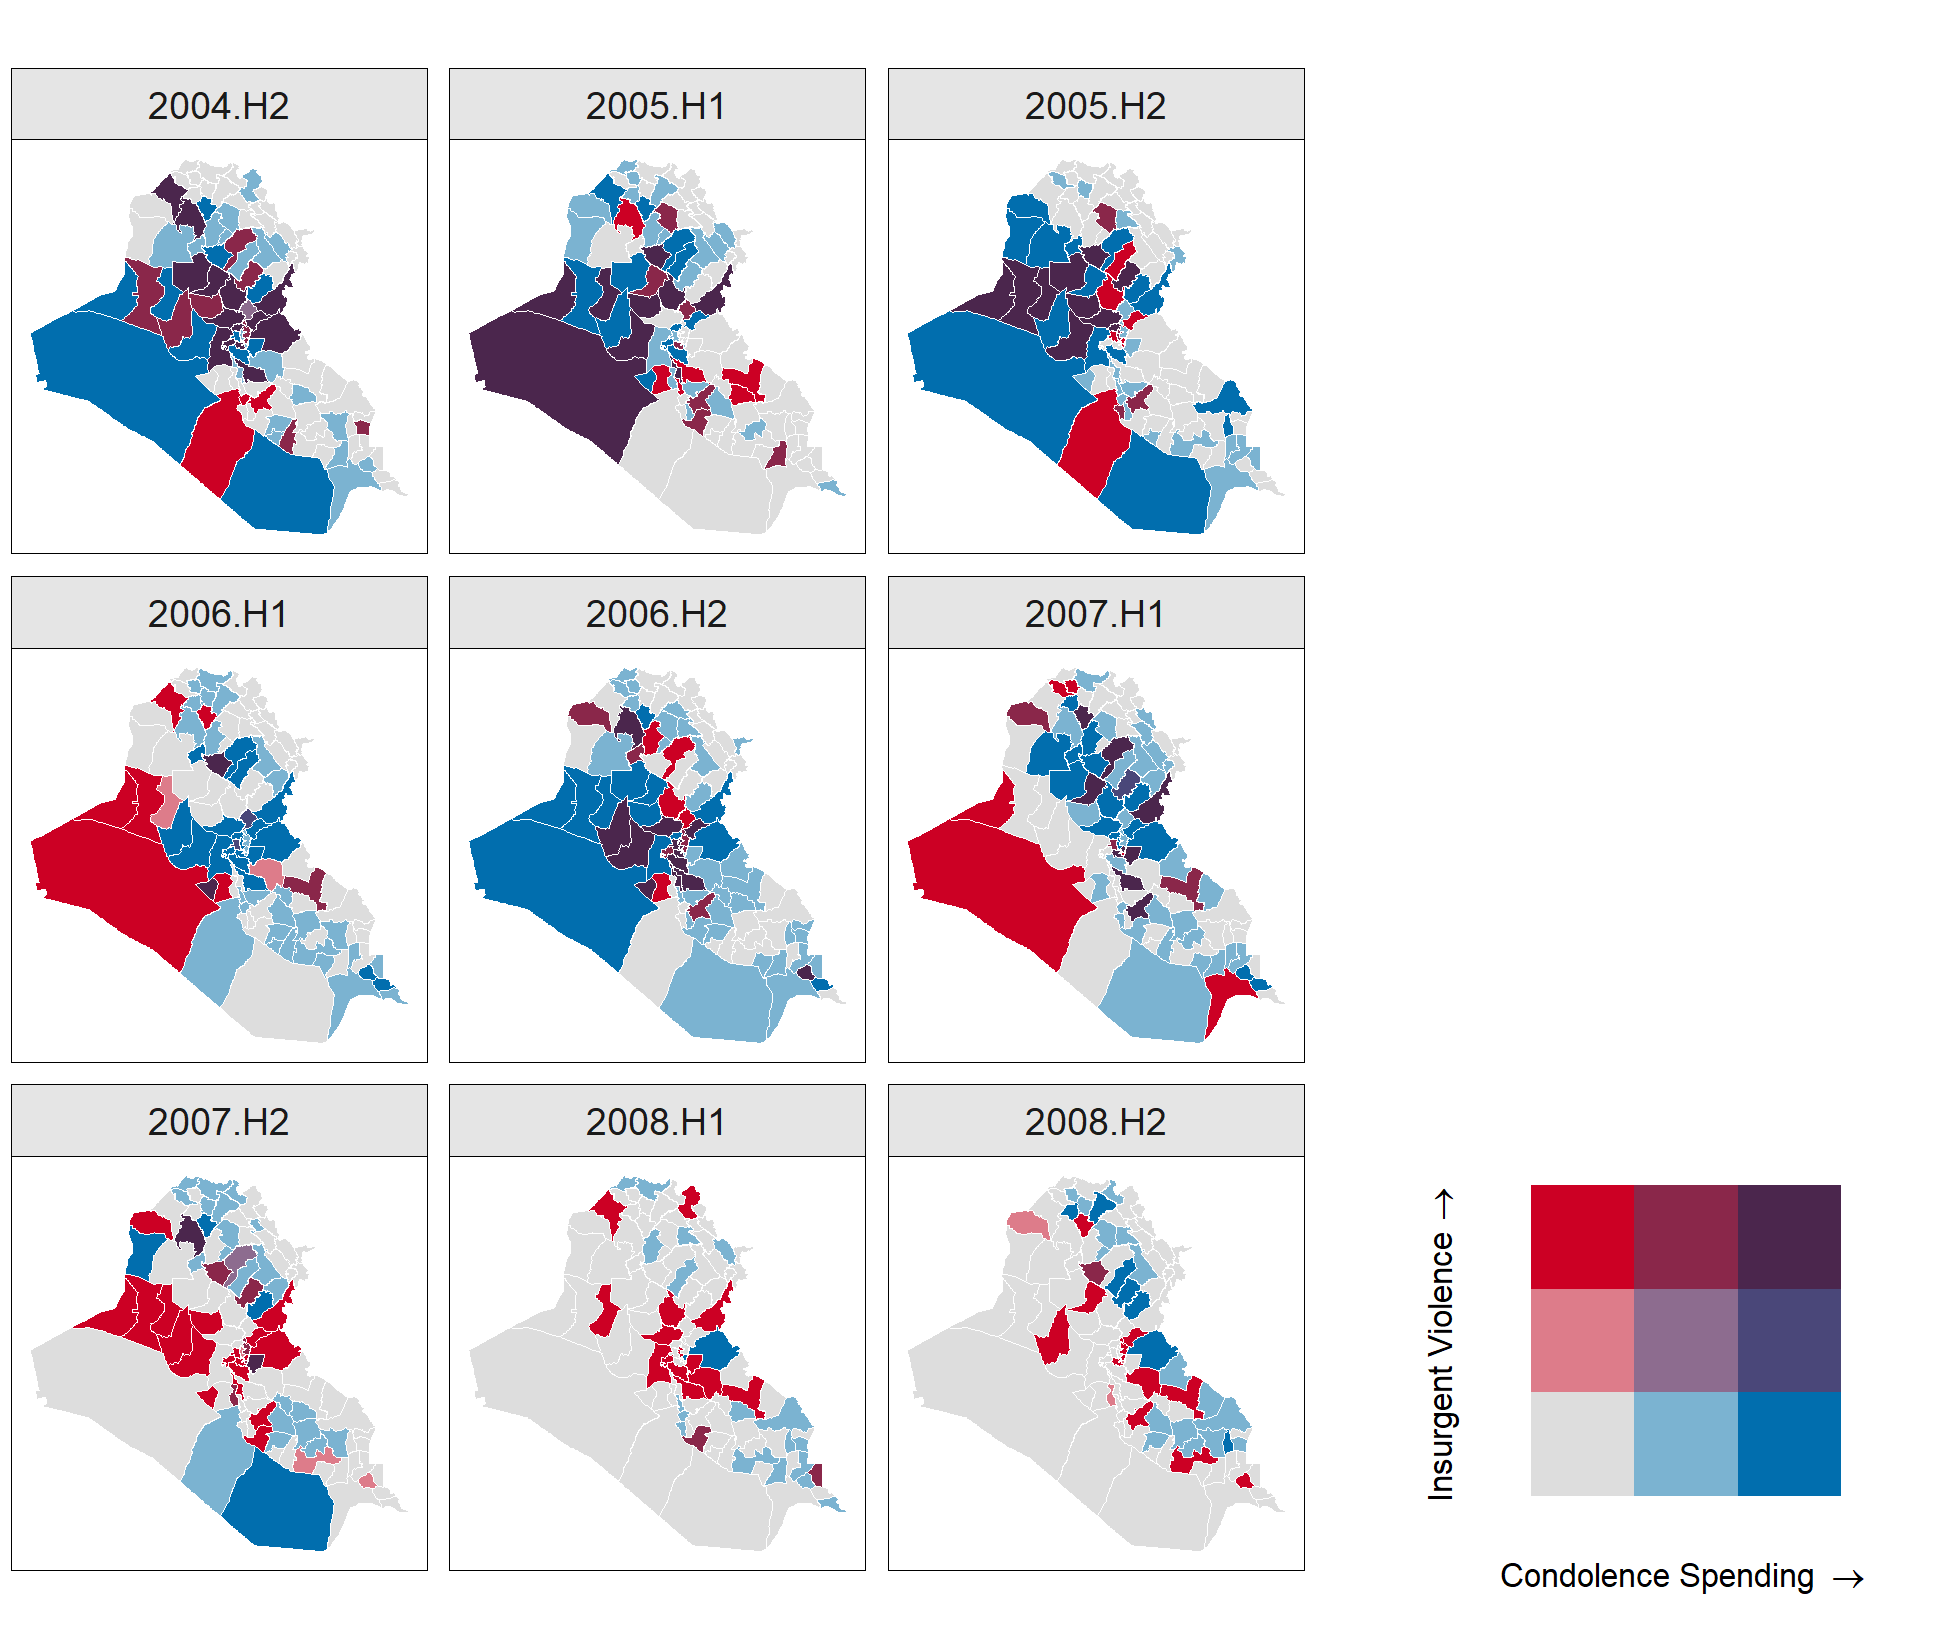
\includegraphics{figure-bimap.png}
  \caption{Bivaraite Map: Insurgent Attacks \& Condolence Spending}
  \label{figure:map_attacks}
\end{figure}

The areas within Iraq that experienced escalating or deescalating violence trends changed over the study period likely due to changing tactical conditions on the ground. In particular, escalating violence in the Al Anbar Governorate in the second-half of 2006 stands out. Insurgent activity appears to demonstrate a clear pattern of diffusion spreading from Iraq's western border in early 2007 eastward by the latter-half of that year before eventually fizzling out. This subsequent pattern of decreasing violence followed the 2007 troop surge and is reflected in the bottom three panes of the figure which reveal fragmented pockets of violence in contrast to earlier violence which covered larger geographic areas. Finally, it also appears that the financial compensation distributed through condolence spending programs lagged behind observed violence with high levels of spending occurring in periods subsequent to periods of higher observed violence.

In the models presented in the following section we begin by first replicating Silverman's published results before presenting the spatio-temporal (STAR) specification and finally the geostatistical spatial models. With the STAR model we follow convention in spatial modeling and employ a row-standardized queen contiguity matrix to define the connections between the units in the data (Franzese and Hays 2007, Anselin 2006). For the Bayesian SPDE models use a combination of default priors used in past research (Python 2018, Lindgren and Rue 2015) while specifying spatial priors that allow us to properly model the spatial scale of the data here. We employ a mesh using district centroids as the triangularization points with a max internal triangular edge length of 0.25 decimal degrees which results in 126 nodes.\footnote{A smaller edge length will increase model precision, but will increase computational cost. 0.25 decimal degrees corresponds to approximately 23.25 miles at Iraq's latitude.}. For parameters on the Mat\'ern correlation function ($\zeta_V$), we employ penalized complexity priors that favor model parsimony and allow us to establish parameter scales consistent with the spatial process under examination here, that is the geographic extent of Iraq. We assign a 10\% probability that:

\begin{itemize}[noitemsep,nolistsep]
  \item the range is above 3.6 (approximately 332 km at Iraq's latitude) $(3.6,\ 0.1)$
  \item the standard deviation is above 1                                $(1.0,\ 0.1)$
\end{itemize}

These priors allow for more variation in the spatial correlation of insurgent violence within Iraq as well as incorporate a theoretically motivated assumption that insurgent events do not significantly influence other such events beyond a large spatial range (332 km). Counterinsurgency efforts as well as US military tactics such as denial of territory commonly employed by combat battalions over the course of the conflict support this contention that insurgents did not influence the activity of other factions beyond this spatial range (CITATION). This prior range further allows us to account for the majority of insurgent activity occurring within Baghdad during this time period and thus the scale of the spatial process implied by the sample of data analyzed here.\footnote{Baghdad's average distance from its nearest international border is approximately 332 km which, at Iraq's latitude, corresponds to the prior value of 3.6 decimal degrees. This prior therefore assigns a small probability that the spatial effects implied by the GRMF extend beyond this range.} On the temporal structure of the GMRF we follow Python et al (2018) and employ a penalized complexity prior where $P(\sigma^2_{rw} > 1 = 0.01)$ implying that the variance of the temporal structure has a low probability of exceeding 1. Finally, we retain \textit{R-INLA} default priors for the fixed effects ($\beta_v$) and unstructured random effects ($\epsilon_V$) which assign i.i.d. zero-mean normal distributions with precision of 0.001.
% ---------------------------------------------------------------------------- %



% ---------------------------------------------------------------------------- %
\section{Statistical Analyses of the External Validity of Machine and Human Coded Data for Iraq}
% ---------------------------------------------------------------------------- %
Table \ref{table:models} contain all model coefficient estimates as well as confidence (credibility) intervals. The first column exactly replicates Silverman's final model following Equation \ref{equation:silverman} with the inclusion of district, time, and Sunni vote-share fixed effects.\footnote{This model appears in Silverman (2021) as the final column of Table 2, p. 866.}. Consistent with the published results, we find that compensation payments significantly reduced the rate of insurgent violence in Iraq over this time period. An additional dollar of condolence spending per capita corresponds to 0.52 fewer insurgent events (-0.88, -0.15) per 1000 residents in a district. Since we include a one-unit time lag of the dependent variable to account for persistence in insurgent activity over time in the STAR and geostatistical models, we lose the first time-unit observations and thus include an identical version of Silverman's model using this subset of data in column 2 - the published results remain substantively and statistically unchanged using these subset data. Condolence spending significantly decreases insurgent violence with an additional dollar spent per capita corresponding to 0.53 fewer insurgent events per 1000 residents in a district.

% ----------------------------------- %
\begin{table}[!h]
\begin{center}
\begin{footnotesize}
\caption{Statistical models}
\label{table:models}
\begin{tabular}{l c c c c}
\toprule
 & \multicolumn{2}{c}{Replication} & \multicolumn{1}{c}{STAR} & \multicolumn{1}{c}{Geostatistical} \\
\cmidrule(lr){2-3} \cmidrule(lr){4-4} \cmidrule(lr){5-5}
 & Published & Subset & STAR-Structural & SPDE \\
\midrule
Condolence Spending (PC)    & $-0.52^{*}$       & $-0.53^{*}$       & $-0.61^{*}$       & $-0.31^{*}$         \\
                            & $ [-0.88; -0.15]$ & $ [-1.00; -0.05]$ & $ [-0.98; -0.25]$ & $ [ -0.61;  -0.02]$ \\
Ruzicka Spending (PC)       & $-0.98^{*}$       & $-1.28^{*}$       & $-0.22$           & $-0.26$             \\
                            & $ [-1.92; -0.04]$ & $ [-2.08; -0.48]$ & $ [-2.21;  1.76]$ & $ [ -1.86;   1.33]$ \\
Coalition Collateral Damage & $0.03^{*}$        & $0.03^{*}$        & $0.05^{*}$        & $0.02^{*}$          \\
                            & $ [ 0.01;  0.04]$ & $ [ 0.01;  0.04]$ & $ [ 0.03;  0.07]$ & $ [  0.01;   0.04]$ \\
Insurgent Collateral Damage & $0.00$            & $-0.00$           & $-0.00$           & $-0.01$             \\
                            & $ [-0.02;  0.02]$ & $ [-0.02;  0.02]$ & $ [-0.02;  0.02]$ & $ [ -0.03;   0.01]$ \\
Other Small CERP Spending   & $-0.18$           & $-0.18$           & $0.26^{*}$        & $0.13$              \\
                            & $ [-0.67;  0.31]$ & $ [-0.71;  0.35]$ & $ [ 0.04;  0.47]$ & $ [ -0.06;   0.32]$ \\
Other USAID Spending        & $-0.00$           & $-0.27$           & $-0.96^{*}$       & $-0.48$             \\
                            & $ [-0.01;  0.00]$ & $ [-0.77;  0.22]$ & $ [-1.63; -0.29]$ & $ [ -1.04;   0.09]$ \\
Coalition Troop Strength    & $0.05$            & $0.05$            & $0.05$            & $0.04$              \\
                            & $ [-0.01;  0.12]$ & $ [-0.03;  0.14]$ & $ [-0.11;  0.20]$ & $ [ -0.08;   0.17]$ \\
CMOC Presence               & $-0.30$           & $-0.33$           & $0.00$            & $0.01$              \\
                            & $ [-0.96;  0.36]$ & $ [-1.13;  0.47]$ & $ [-0.19;  0.19]$ & $ [ -0.16;   0.17]$ \\
PRT Presence                & $0.01$            & $0.01$            & $-0.08$           & $-0.04$             \\
                            & $ [-0.19;  0.21]$ & $ [-0.23;  0.25]$ & $ [-0.30;  0.14]$ & $ [ -0.24;   0.17]$ \\
Phi                         &                   &                   & $0.17^{*}$        & $0.08^{*}$          \\
                            &                   &                   & $ [ 0.10;  0.23]$ & $ [  0.02;   0.13]$ \\
Rho                         &                   &                   & $0.36^{*}$        &                     \\
                            &                   &                   & $ [ 0.28;  0.45]$ &                     \\
Kappa                       &                   &                   &                   & $1.52^{*}$          \\
                            &                   &                   &                   & $ [  1.06;   2.04]$ \\
Sigma$^2$                   &                   &                   &                   & $0.65^{*}$          \\
                            &                   &                   &                   & $ [  0.40;   0.95]$ \\
Range (km)                  &                   &                   &                   & $207.09^{*}$        \\
                            &                   &                   &                   & $ [146.23; 280.37]$ \\
\midrule
FE: District                & Yes               & Yes               & No                & No                  \\
FE: Time                    & Yes               & Yes               & No                & No                  \\
FE: Sunni VS                & Yes               & Yes               & No                & No                  \\
n                           & $927$             & $824$             & $824$             & $824$               \\
LogLik                      & $-1109.50$        & $-1011.66$        & $-1166.25$        & $-890.19$           \\
AIC                         & $2477.00$         & $2277.32$         & $2356.50$         & $2314.57$           \\
BIC                         & $3100.32$         & $2876.02$         & $2413.07$         & $3573.70$           \\
\bottomrule
\multicolumn{5}{l}{\tiny{$^*$ Null hypothesis value outside the confidence (credibility) interval.}}
\end{tabular}
\end{footnotesize}
\end{center}
\end{table}
% ----------------------------------- %

NOTE - may want to mention that Coalition collateral damage is consistently estimated across all models providing some degree of assurance that, for variables with a strong signal, the spatial modeling choices here does not negatively impact results.

These estimates in these fixed-effects models, however, make no provision for dynamic feedback effects which theoretically are likely to manifest in the relationship between condolence spending and insurgent violence.\footnote{Lagrange Multiplier robust test statistics strongly support a spatial lag process in both replication models presented in Table \ref{table:models}.} Seeing coalition military forces make conciliatory gestures towards their neighbors, civilians in nearby regions should be more likely to share information with coalition forces in their districts leading to spatial effects whereby condolence dollars spent in one region have downstream effects in neighboring regions. To account for this we now turn to the dynamic models.

Turning to the STAR model estimates in column 3, the spending coefficient is consistent in magnitude with the fixed-effects models: an additional per capita dollar in compensation spending leads to a pre-spatial, pre-temporal impulse reduction in insurgent attacks of -0.61 (-0.98, -0.25). However, the STAR model provides strong evidence of spatial and temporal multipliers as both Phi and Rho are highly significant and positive indicating positive spatial and temporal autocorrelation. This provides evidence against the assumption of localized violence in the Iraq conflict space made with fixed-effects models. Solving the reduced-form version of the model allow us to capture these causal mechanisms and estimate the long-run-steady-state (LRSS) equilibrium responses to unit-changes condolence spending (and all other exogenous variables) on insurgent activity (Franzese and Hays, 2007; Anselin, 2006).

% ----------------------------------- %
\begin{table}[!h]
\begin{center}
\begin{footnotesize}
\caption{STAR - LRSS}
\label{table:star_reduced}
\begin{tabular}{l c}
\toprule
 & STAR-LRSS \\
\midrule
Condolence Spending (PC)    & $-1.30^{*}$       \\
                            & $ [-2.20; -0.53]$ \\
Ruzicka Spending (PC)       & $-0.51$           \\
                            & $ [-4.85;  3.98]$ \\
Coalition Collateral Damage & $0.10^{*}$        \\
                            & $ [ 0.06;  0.16]$ \\
Insurgent Collateral Damage & $-0.01$           \\
                            & $ [-0.05;  0.03]$ \\
Other Small CERP Spending   & $0.52^{*}$        \\
                            & $ [ 0.07;  1.00]$ \\
Other USAID Spending        & $-2.04^{*}$       \\
                            & $ [-3.71; -0.70]$ \\
Coalition Troop Strength    & $0.11$            \\
                            & $ [-0.23;  0.40]$ \\
CMOC Presence               & $0.00$            \\
                            & $ [-0.39;  0.41]$ \\
PRT Presence                & $-0.17$           \\
                            & $ [-0.65;  0.29]$ \\
\bottomrule
\multicolumn{2}{l}{\tiny{$^*$ 0 outside the confidence interval.}}
\end{tabular}
\end{footnotesize}
\end{center}
\end{table}
% ----------------------------------- %

We present these LRSS estimates in Table \ref{table:star_reduced}. After accounting for the feedback effects across space and over time, we can see that each dollar spent in compensation by coalition forces yields large downstream returns in terms of reduction in insurgent activity: an additional dollar per capita in condolence spending reduces insurgent attacks per 1000 people by 1.30 (-2.20, -0.53) within a district. This dynamic effect is 1.8 times the magnitude of the effect reported in the fixed-effects model. While the STAR model presented here better captures theoretically implied feedback effects between compensation spending and violence, it does so by imposing a strong assumption on the relationships between units in the data: a step-function for neighbor contiguity. By making this assumption, we cannot estimate the range at which violence correlates with itself before decaying and having no substantive influence on conflict processes at more distant locations. To better understand this process of decay across space, we turn to the final geostatistical model presented in Table \ref{table:models}.

In contrast to the STAR model with a spatial dynamic process in the structural form of the model, in our geostatistical model we model spatial dependence as a continuous latent process in a Gaussian Markov Random Field fit with a stochastic partial differential equation that yields estimates of the range of spatial correlation as well as field variance. Relative to the fixed-effects setup, the estimate of the pre-temporal\footnote{Note that we retain the temporal lag, Phi, in the model.} impulse is smaller in magnitude, yet consistent in the negative direction while remaining reliably non-zero based on the 95\% credibility interval. The final three estimates in column 4: Kappa, $Sigma^2$, and Range describe the Gaussian field characterizing insurgent activity in Iraq over this time period. Most importantly, we are able to estimate a value of the range at which the spatial correlation between insurgent events becomes negligible: 207 km (146, 280). The median distance from Iraqi district centroids to their borders is 26km (95\% quantile: [11, 76]), therefore this estimated value for the range of spatial correlation in insurgent activity further reinforces a non-localized conflict process whereby violence diffuses across district borders.

\begin{figure}[!h]
  \centering
  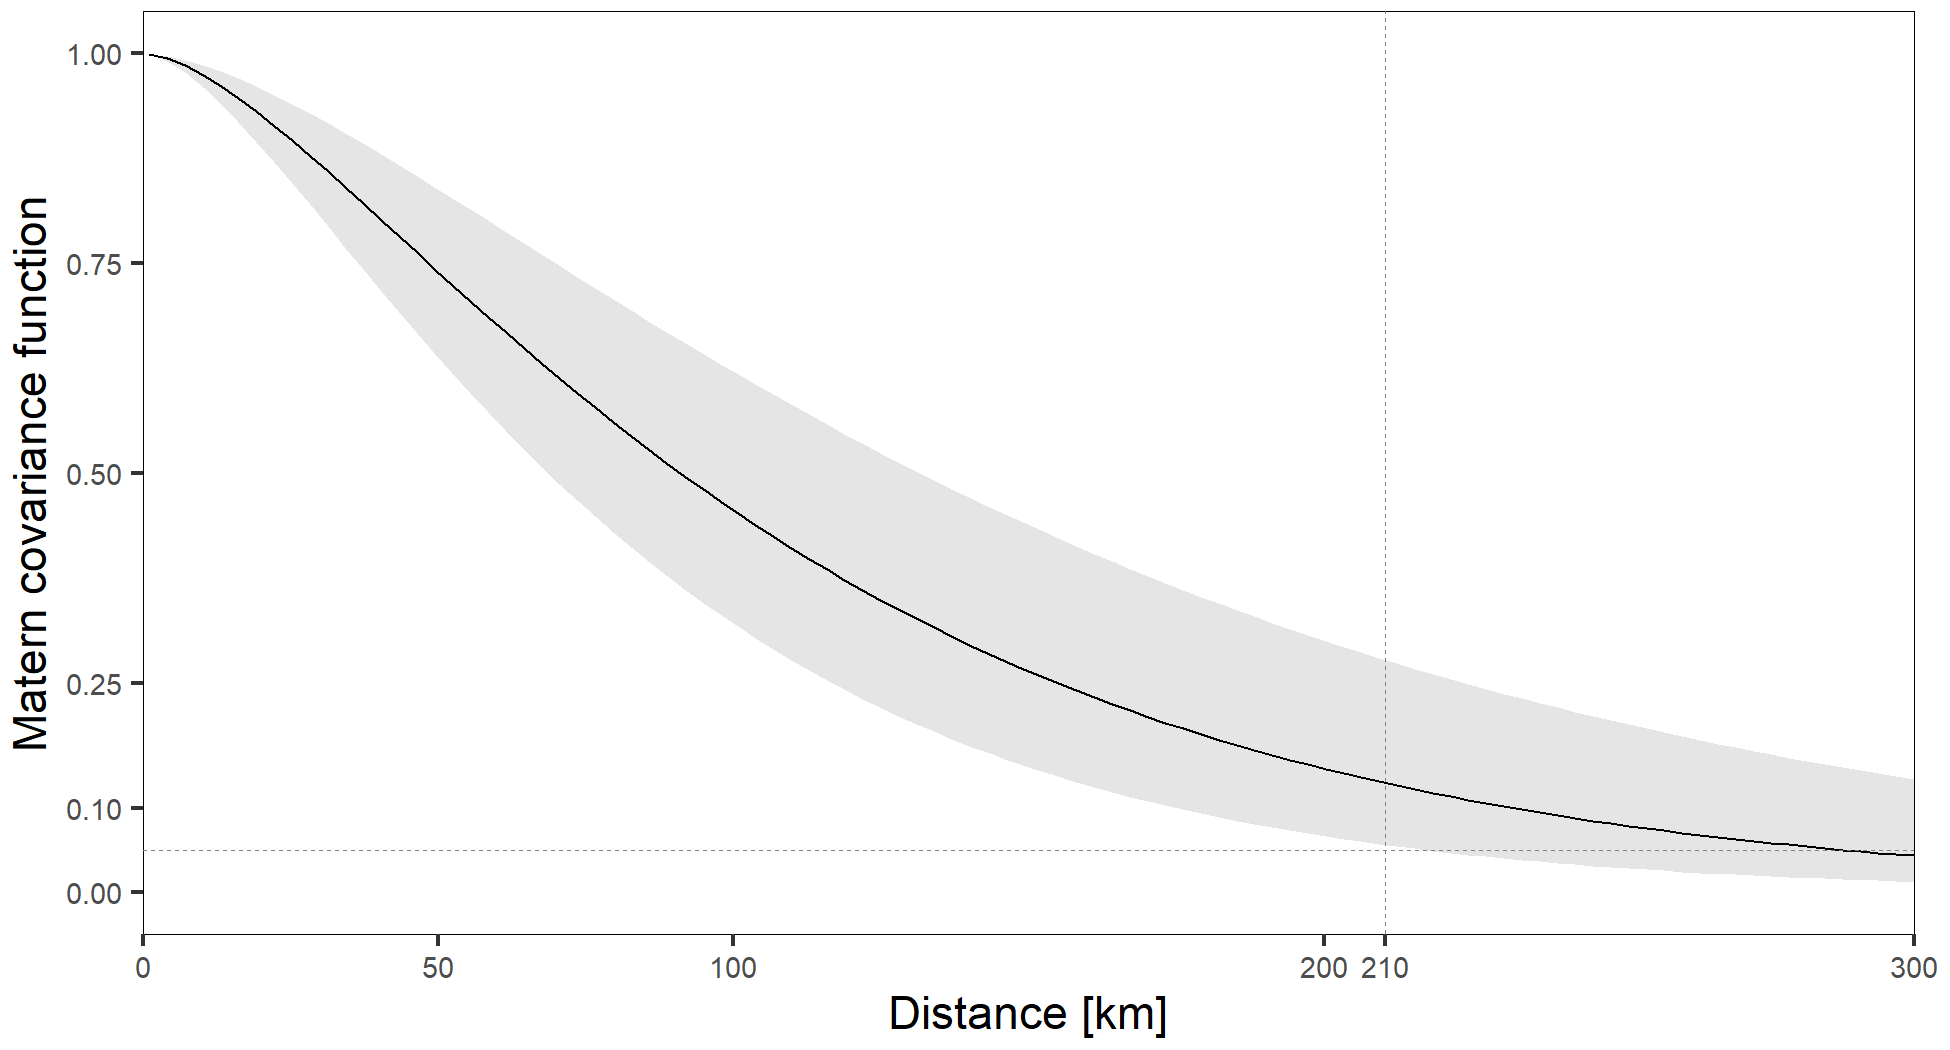
\includegraphics{figure-spde_range.png}
  \caption{SPDE Range Estimates - Spatial correlation of insurgent activity}
  \label{figure:spde_range}
\end{figure}

Figure \ref{figure:spde_range} visualizes the spatial decay in the spatial correlation of insurgent attacks across the GMRF. A spatially isolated process which occurs locally within districts and does \textit{not} exhibit escalation diffusion or escalation relocation would exhibit a sharp and rapid decay in the spatial correlation of insurgent events as the distance from an event increased across space. In contrast a local process of that nature, here we observe the decay of spatial correlation exhibits persistence where the influence of events extends steadily beyond the boundaries of an average Iraqi district thereby exerting influence on events in neighbors and beyond.

\begin{figure}[!h]
  \centering
  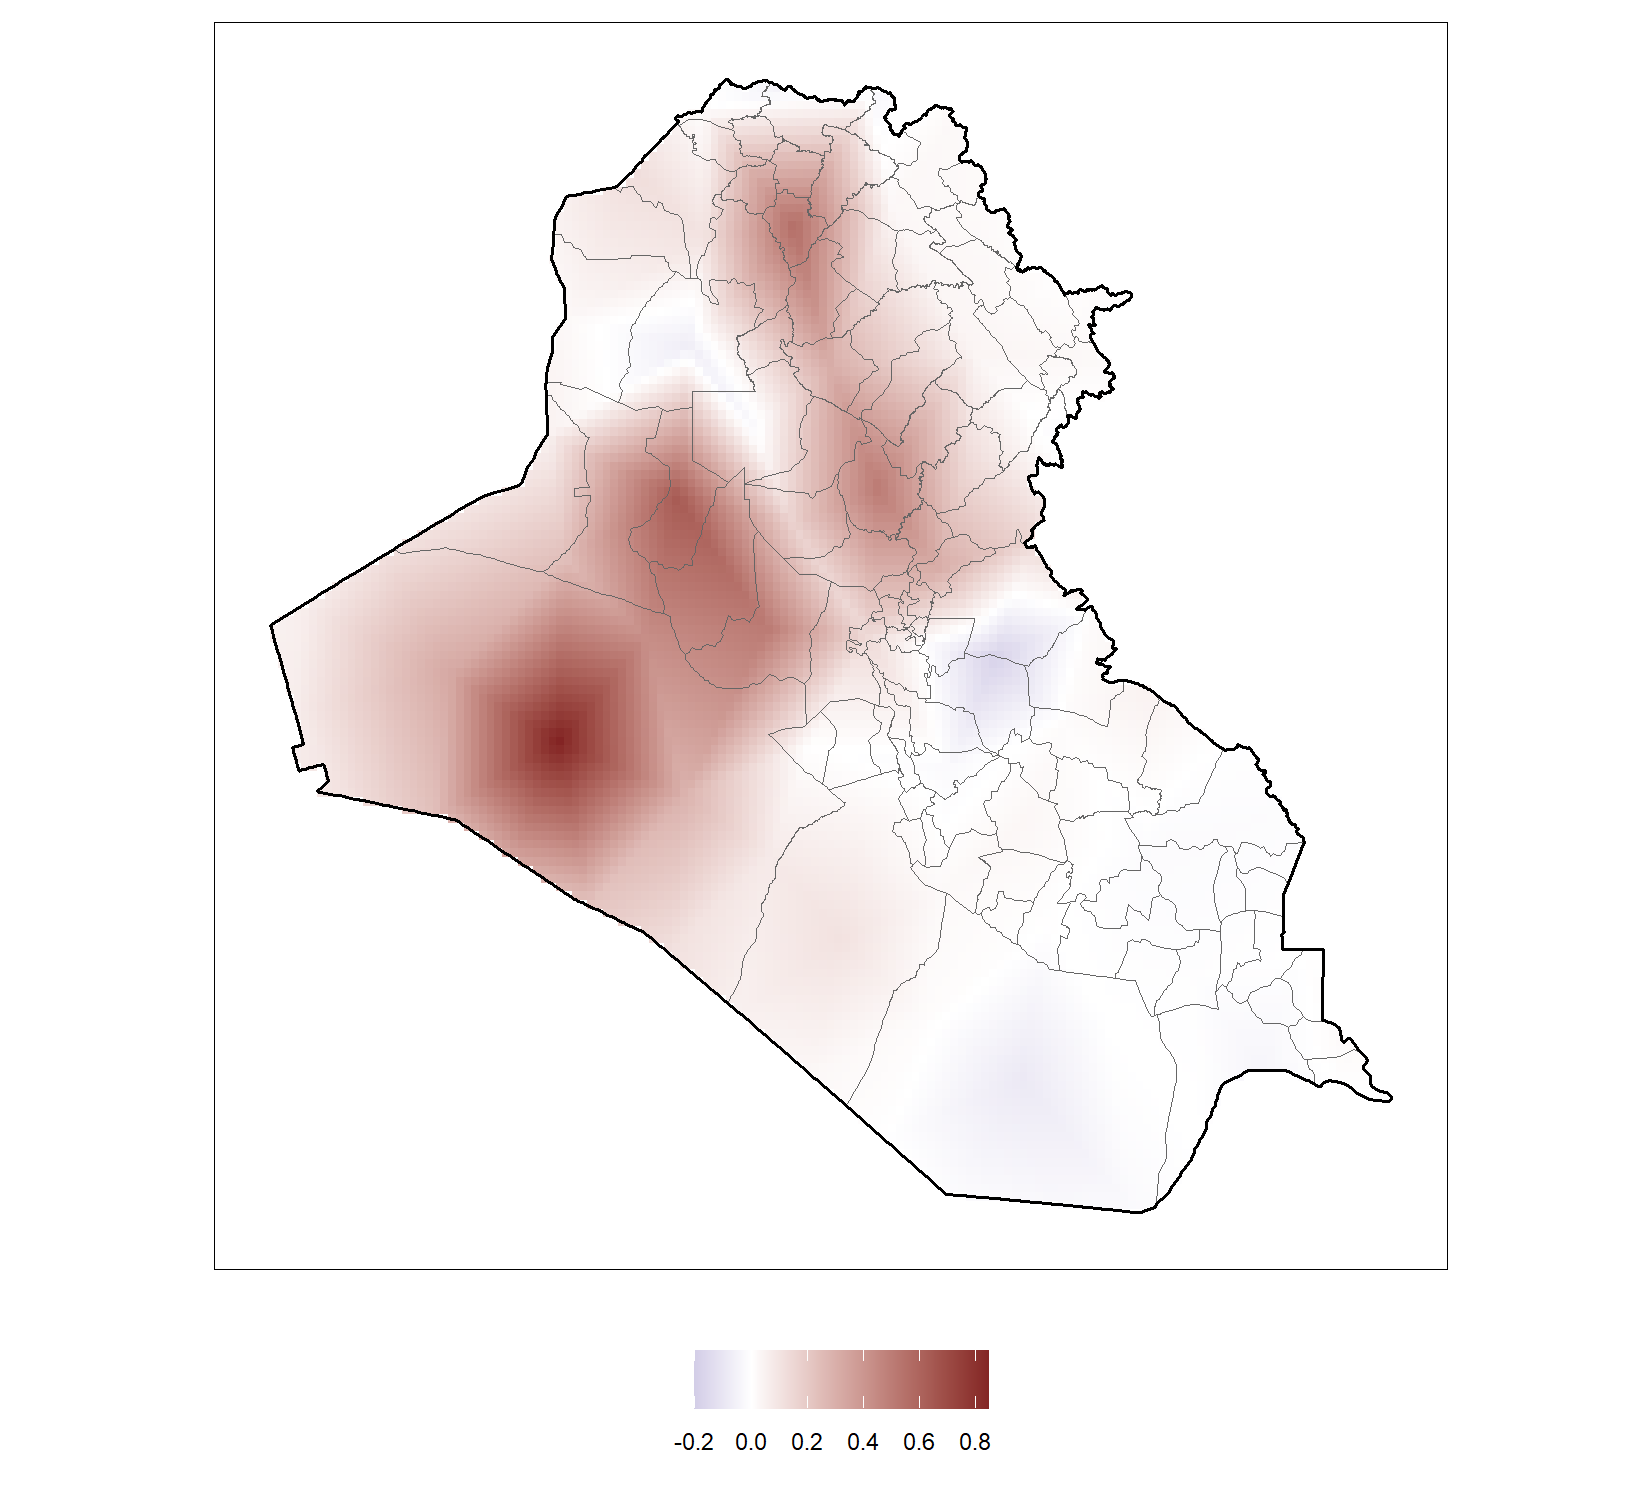
\includegraphics{figure-gmrf_mean.png}
  \caption{GMRF $\zeta$, Mean Estimates}
  \label{figure:map_gmrf}
\end{figure}

Site-specific estimates of the Gaussian Field can be mapped onto the estimation mesh to visualize locations of higher(lower) estimated insurgent activity across the continuous spatial domain used to fit the geostatistical model. Figure \ref{figure:map_gmrf} presents these estimates and reveals regions where high and lower levels of insurgent activity persisted over the course of the conflict. The Al Anbar region in the West stands out as a clear hot-spot of insurgent activity as does the dividing line between Kurdish and Sunni regions in the country's Northeast region. What emerges from these field estimates is the clear evidence of diffusion of insurgent activity across district boundaries. This further implies that the decision of insurgents engage in acts of violence depended upon more than local factors alone either modeled as observable covariates or through the inclusion of unit and time fixed-effects. While local factors matter, these results make clear that nearby insurgent activity - up to a distance of 207 km (146, 280) significantly matters for explaining this conflict process.


% ----------------------------------- %
% Logan's new results for effects of compensation when allowing for unit invariant
% persistence in form of lagged dependent variable. Does this hold up with ICEWS
% and GED? Footnote Blair (2021) use of STAR as robustness checks and flaws
% in his STAR application

% Admit to temporal discretization ala Cseke et al. 1747 top col 2. The effects of the localization assumption in Silverman ought to be illuminated in a way not revealed by the STAR model.
% ----------------------------------- %
% ---------------------------------------------------------------------------- %



% ---------------------------------------------------------------------------- %
\section{Conclusion}
% ---------------------------------------------------------------------------- %

Here we have discussed and presented three approaches to accounting for space and time in our modeling of social theory: commonly employed fixed effects models, less-common dynamic spatiotemporal models which leverage pre-specified connectivity matrices, and novel geostatistical techniques which make no \textit{a priori} assumptions about the connections between units but rather estimate connections as a function of observed data. Using recent studies of political violence and armed conflict as an illustration, the results we have presented here demonstrate that the common approaches to treating space and time as ''nuisances" to control away leave much to be desired and miss important theoretical processes underpinning the connection between theoretically relevant variables and our outcomes of interest.

Note ubiquitous spatiotemporal processes across political science (American legislators casting votes in congress, diffusion of policy across state borders, unemployment shocks or trade shocks, etc... \\

\begin{itemize}[noitemsep,nolistsep]
  \item future work:
  \item non-separable space time
  \item non-stationary spatial processes
  \item continuous time domain spatial spde models - Cseke et al. here but also Krainski et al. Adv. Spatial Modeling with SPDE Ch. 7
\end{itemize}


% ---------------------------------------------------------------------------- %
























% ---------------------------------------------------------------------------- %
\newpage
\singlespace
\section{References}
% ---------------------------------------------------------------------------- %

\bibitem Anselin, Luke 2006. "Spatial Econometrics" Chapter 26 in
 \emph{Palgrave Handbook of Econometrics} Volume 1. Econometrics. Basingstone,
 Palgrave MacMillon, pps. 901-969

\bibitem Bandyopadhyay, Soutir, and S.S. Rao. 2017.
  ``A Test for Stationarity in Irregularly Spaced Data."
\emph{Journal of the Royal Statistical Society} 79(1): 95-123.

\bibitem Bagozzi, Benjamin E., Patrick T Brandt, John R. Freeman, A, Kim, A. Palao,
  and Carly Potz-Nielsen. 2018 " The Prevalence and Severity of Underreporting Bias
   in Machine and Human Coded Data" \emph{Political Science Research and Methods}
  7(3): 641-649.

\bibitem Berman Eli, Michael Callen, Joseph H. Felter and Jacob Shapiro. 2011.
 "Do Working Men Rebel? Insurgency in Afghanistan, Iraq, and the Philippines."
 \emph{Journal of Conflict Resolution} 55(4): 496-528

\bibitem Berman Eli, Joseph Felter, Jabob Shapiro. 2018. \emph{Small Wars, Big Data: The Information Revolution in Modern Conflict}. Princeton, Princeton University Press.

\bibitem Biddle, Stephen, Jeffrey A. Friedman, and Jacob N. Shapiro. 2020.
 "Testing the Surge: Why Did Violence Decline in Iraq in 2007? \emph{International
 Security} 37(1): 7-40.

\bibitem Blair, Christopher W. 2021 "Restitution or Retribution? Detainee Payments
 and Insurgent Violence" Unpublished Manuscript. State College, PA.

\bibitem Blangiardo, Marta and Michela Cameletti. 2015. \emph{Spatial and
 Spatial-temporal Bayesian Models with R-INLA} New York, John Wiley and Sons.

\bibitem Box-Steffensmeier, Janet, John R. Freeman, Matthew P. Hitt, and
 Jon C. Pevehouse. 2014. \emph{Time Series Analysis for the Social Sciences}
 New York. Cambridge U

\bibitem Braithwaite, Alex and Shane D. Johnson. 2012 "Space-Time Modeling of
 Insurgency and Counterinsurgency in Iraq" \emph{Journal of Quantitative Criminology}
 28: 31-48.

\bibitem Brandt, Patrick T., John R. Freeman and Philip Schrodt. 2014.
"Evaluating Forecasts of Political Conflict Dynamics."
 \emph{International Journal of Forecasting} 30(4): 944-962.

\bibitem Brandt, Patrick T., Michael Colaresi, and John R. Freeman 2008.
"The Dynamics of Reciprocity, Accountability, and Credibility."
 \emph{Journal of Conflict Resolution} 52(3): 343-374.

\bibitem Cameletti, Michela, Rosaria Ignaccolo, and Stefano Bande. 2011
"Comparing Spatio-temporal models for Particulate Matter in the Piemonte."
 \emph{Environmentrics} 22: 985-996.

\bibitem Center for Army Analysis. Deployed Analyst History Report--Volume 1.
 Analytic Support to Combat Operations in Iraq 2002-2011. 2012 Fort Belvoir, Virginia.

\bibitem Cseke, Botond, Andrew Zammit-Mangion, Tom Heskes, and Guido Sanguinetti. 2016.
``Sparse Approximate Inference for Spatio-Temporal Point Process Models."
\emph{Journal of the American Statistical Association}" 111(516)" 1746-1763.

\bibitem Cho, Wemdy K. "Contagion Effects and Ethnic Contribution Networks"
\emph{American Journal of Political Science} 47(2): 368-387.

\bibitem Cho, Wendy K. and James G. Gimpel. 2003 "Prospecting for Gold"
\emph{American Journal of Political Science} 51(2): 255-268.

\bibitem Condra, Luke N. and Jacob N. Shapiro. 2012 "Who Takes the Blame?
The Strategic Effects of Collateral Damage" \emph{American Journal of Political
Science} 56(1): 167-187.

\bibitem Donnay, Karsten and Vladimir Filmanov. 2014. "Views to a War: Systematic
Differences in Media and Military Reporting of the War in Iraq"
\emph{EPJ Data Science} 3 XXX

\bibitem Enders, Walter. 2010. \emph{Applied Econometric Time Series} Third
 Edition. New York, Wiley.

\bibitem Franzese, Robert Jr., Jude C. Hays, and Scott J. Cook. 2015.
 "Spatial and Spatial-temporal-Autoregressive Probit Models of Interdependent
 Binary Outcomes." \emph{Political Science Research and Methods} 4(1): 151-173.

\bibitem Franzese, Robert Jr. and Jude C. Hays. 2007.
"Spatial-Econometric Models of Cross-Section Interdependence in Political Science
 Panel and Time Series Cross Section Data." \emph{Political Analysis} 15(2): 140-164.

 \bibitem Gill 2020.XXXX

\bibitem Gneiting, Thomas. 2002 "Nonseparable, Stationary Covariance Functions
for Space-Time Data" \emph{Journal of the American Statistical Association}
97(458): 590-600

\bibitem Hagan, John, Joshua Kaiser, and Anna Hanson. 2016. \emph{American Sociological
Review} 81(2): 316-346.

\bibitem Hammond, Jesse and Nils B. Weidmann. 2014. "Using Machine Coded Even Data
for the Micro-level Study of Political Violence" \emph{Reaearch and Politics}
July-September: 1-6.

\bibitem Imai,Kosuke, and InSong Kim 2020. "On the Use of Two-Way Fixed Effects Regression
Models for Causal Inference with Panel Data."
\emph{Political Analysis} 29: 405-415

\bibitem Imai, Kosuke, and InSong Kim 2019 "When Should We Use Unit Fixed Effects
Regression Models for Causal Inference with Longitudinal Data?"
\emph{American Journal of Political Science} 63(2): 467-490.

\bibitem Ingebrigtsen, R., F. Lindgren, I. Steinsland, and S. Martino. 2015.
``Estimation of a Nonstationary Model of for Annual Participation in Southern
 Norway Using Replicates of the Spatial Field." \emph{Spatial Statistics}C 14: 338-364.

\bibitem Harvill, Jane L. 2010 "Spatio-temporal Processes."
wires.wiley. com/compstats. vol 2: 376-382

\bibitem Jun, and Scott Cook 2020.

\bibitem Keele, Luke and Rocio Titiunik. 2015. "Geographic Boundaries as
Regression Discontinuities." \emph{Political Analysis} 23: 127-155.

\bibitem Keele, Luke and William Minozzi. 2013. "How Much is Minnesota
Like Wisconain? Assumptions and Inference in Observational Data."
\emph{Political Analysis} 21(2): 193-216

\bibitem Linke, Andrew M., Frank W. Witmer, and John O`Loughlin. 2012.
"Space Time Granger Analysis of the War in Iraq: A Study of Coalition
and Insurgent Action-Reaction" \emph{International Interactions} 38: 402-425.

\bibitem Lindgren, F. and H. Rue. 2015. "Bayesian Spatial and Spatial-Temporal
 Modeling with R-INLA." \emph{Journal of Statistical Software} 63(19).

\bibitem Lindgren, F., H. Rue, and J. Lindstrom. 2011. "An Explicit Link Between
 Gaussian fields and Gaussian Markov Random Fields. The Stochastic Differential
 Equation Approach (with Discussion)." \emph{Journal of the Royal Statistical
 Society} Series B 73(4): 423-498

\bibitem Martinelli, D. and G. Geniaux. 2017 "Approximate Likelihood Estimation
 of Spatial Probit Models" \emph{Regional Science and Urban Economics}
 64: 30-45.

\bibitem Monogan III, J.E. and Jeff Gill 2015. "Measuring State and District
 Level Ideology With Spatial Realignment." \emph{Political Science Research
  and Methods} 4(1): 97-121.

\bibitem Pavia, Jose Manuel, Beatriz Larraz, and Jose Maria Montero. 2008.
 "Election Forecasts Using Spatiotemporal Models" \emph{Journal of the
 American Statistical Association} 103(483): 1050-1059

\bibitem Python, A., J.B. Illian, C.M. Jones-Todd, and M.Blangiardo. 2018.
"A Bayesian Approach to Modeling Subnational Spatial Dynamics of World
 Wide Non-state Terrorism, 2010-2016." \emph{Journal of the Royal Statistical
 Society} Series A pps. 1-22.

\bibitem Python, A., J. Illian, C. Jones-Todd, and M. Blangiardo. 2017.
"Explaining the Lethality of Boko Haram's Terrorist Attacks in Nigeria,
2009-2014." In \emph{Bayesian Statistics in Action} R.Argento et al.
eds. Springer.

\bibitem Schutte, Sebastian and Karsten Donnay. 2014. "Matched Wake Analysis:
Finding Causal Relationships in Spatiotemporal Data" \emph{Political Geography}
41: 1-10.

\bibitem Schutte, Sebastian and Nils Weidmann. 2011.
``Diffusion Patterns of Violence in Civil Wars."
\emph{Political Geography} 30: 143-152.

\bibitem Shapiro, Jacob N. and Nils B. Weidmann 2015. "Is the Phone Mightier
Than the Sword? Cellphones and Insurgent Violence in Iraq" \emph{International
Organization} 69: 247-274

\bibitem Silverman, Daniel 2021. "Too Late to Apologize? Collateral Damage,
  Post-Harm Compensation, and Insurgent Violence in Iraq." \emph{International
  Organization} XX

\bibitem Stundal, Logan, Benjamin E. Bagozzi, John R. Freeman, and Jennifer S. Holmes.
  forthcoming. "Human Rights in Space: Statistical Modelss of Machine Coded vs. Human Coded Data."
  \emph{Political Analysis}

\bibitem vonBorzykowski, Inkenand Michael Wahman. 2021  "Systematic Measurement Error
in Election Violence Data: Causes and Consequences." \emph{British Journal of Political
Science} XXX

\bibitem Ward, Michael D. and Kristian Skrede Gleditsch. 2019 \textit{Spatial Regression
Models} Second Edition. Los Angeles California. Sage Publications.

\bibitem Ward, Michael D. and Kristian Skrede Gleditsch. 2002. "Location, Location,
 Location. A MCMC Approach to Modeling the Spatial Context of War and Peace."
 \emph{Political Analysis} 10(3): 244-260.

\bibitem Weinstein, Jeremy. 2007. \emph{Inside Rebellion}. Cambridge, Cambridge University Press.

\bibitem Weidmann, Nils B. and Michael Ward. 2010. "Predicting Conflict in Space and
 Time" 2010. \emph{Journal of Conflict Resolution} 54(6): 883-901

\bibitem Zammit-Mangion, Andrew, Michael Dewar, Visakan Kadirkamanathan, and Guido
Sanguinetti. 2012. "Point Process Modeling of the Afgan War Diary". \emph{PNAS}
109(31): 12414-12419.

\end{document}
